\section{Software Layers}
\label{sec:sad-layers}

In diesem Abschnitt werden die verschiedenen Ebenen der Architektur der Beispielapplikation beschrieben.

Um einen grundsätzlichen Einblick zu erhalten wird jede Ebene zuerst komplett unabhängig von jeglicher konkreter Technologie vorgestellt. In einem weiteren Schritt werden die verwendeten Technologien eingeführt und kurz erläutert.


\subsection*{Technologieneutral}

\begin{figure}[H]
	\centering{
		% Graphic for TeX using PGF
% Title: /Users/michael/code/BA/dokumentation/content/sad/diagrams/layers-diagram.dia
% Creator: Dia v0.97.2
% CreationDate: Wed Jun 12 08:06:39 2013
% For: michael
% \usepackage{tikz}
% The following commands are not supported in PSTricks at present
% We define them conditionally, so when they are implemented,
% this pgf file will use them.
\ifx\du\undefined
  \newlength{\du}
\fi
\setlength{\du}{15\unitlength}
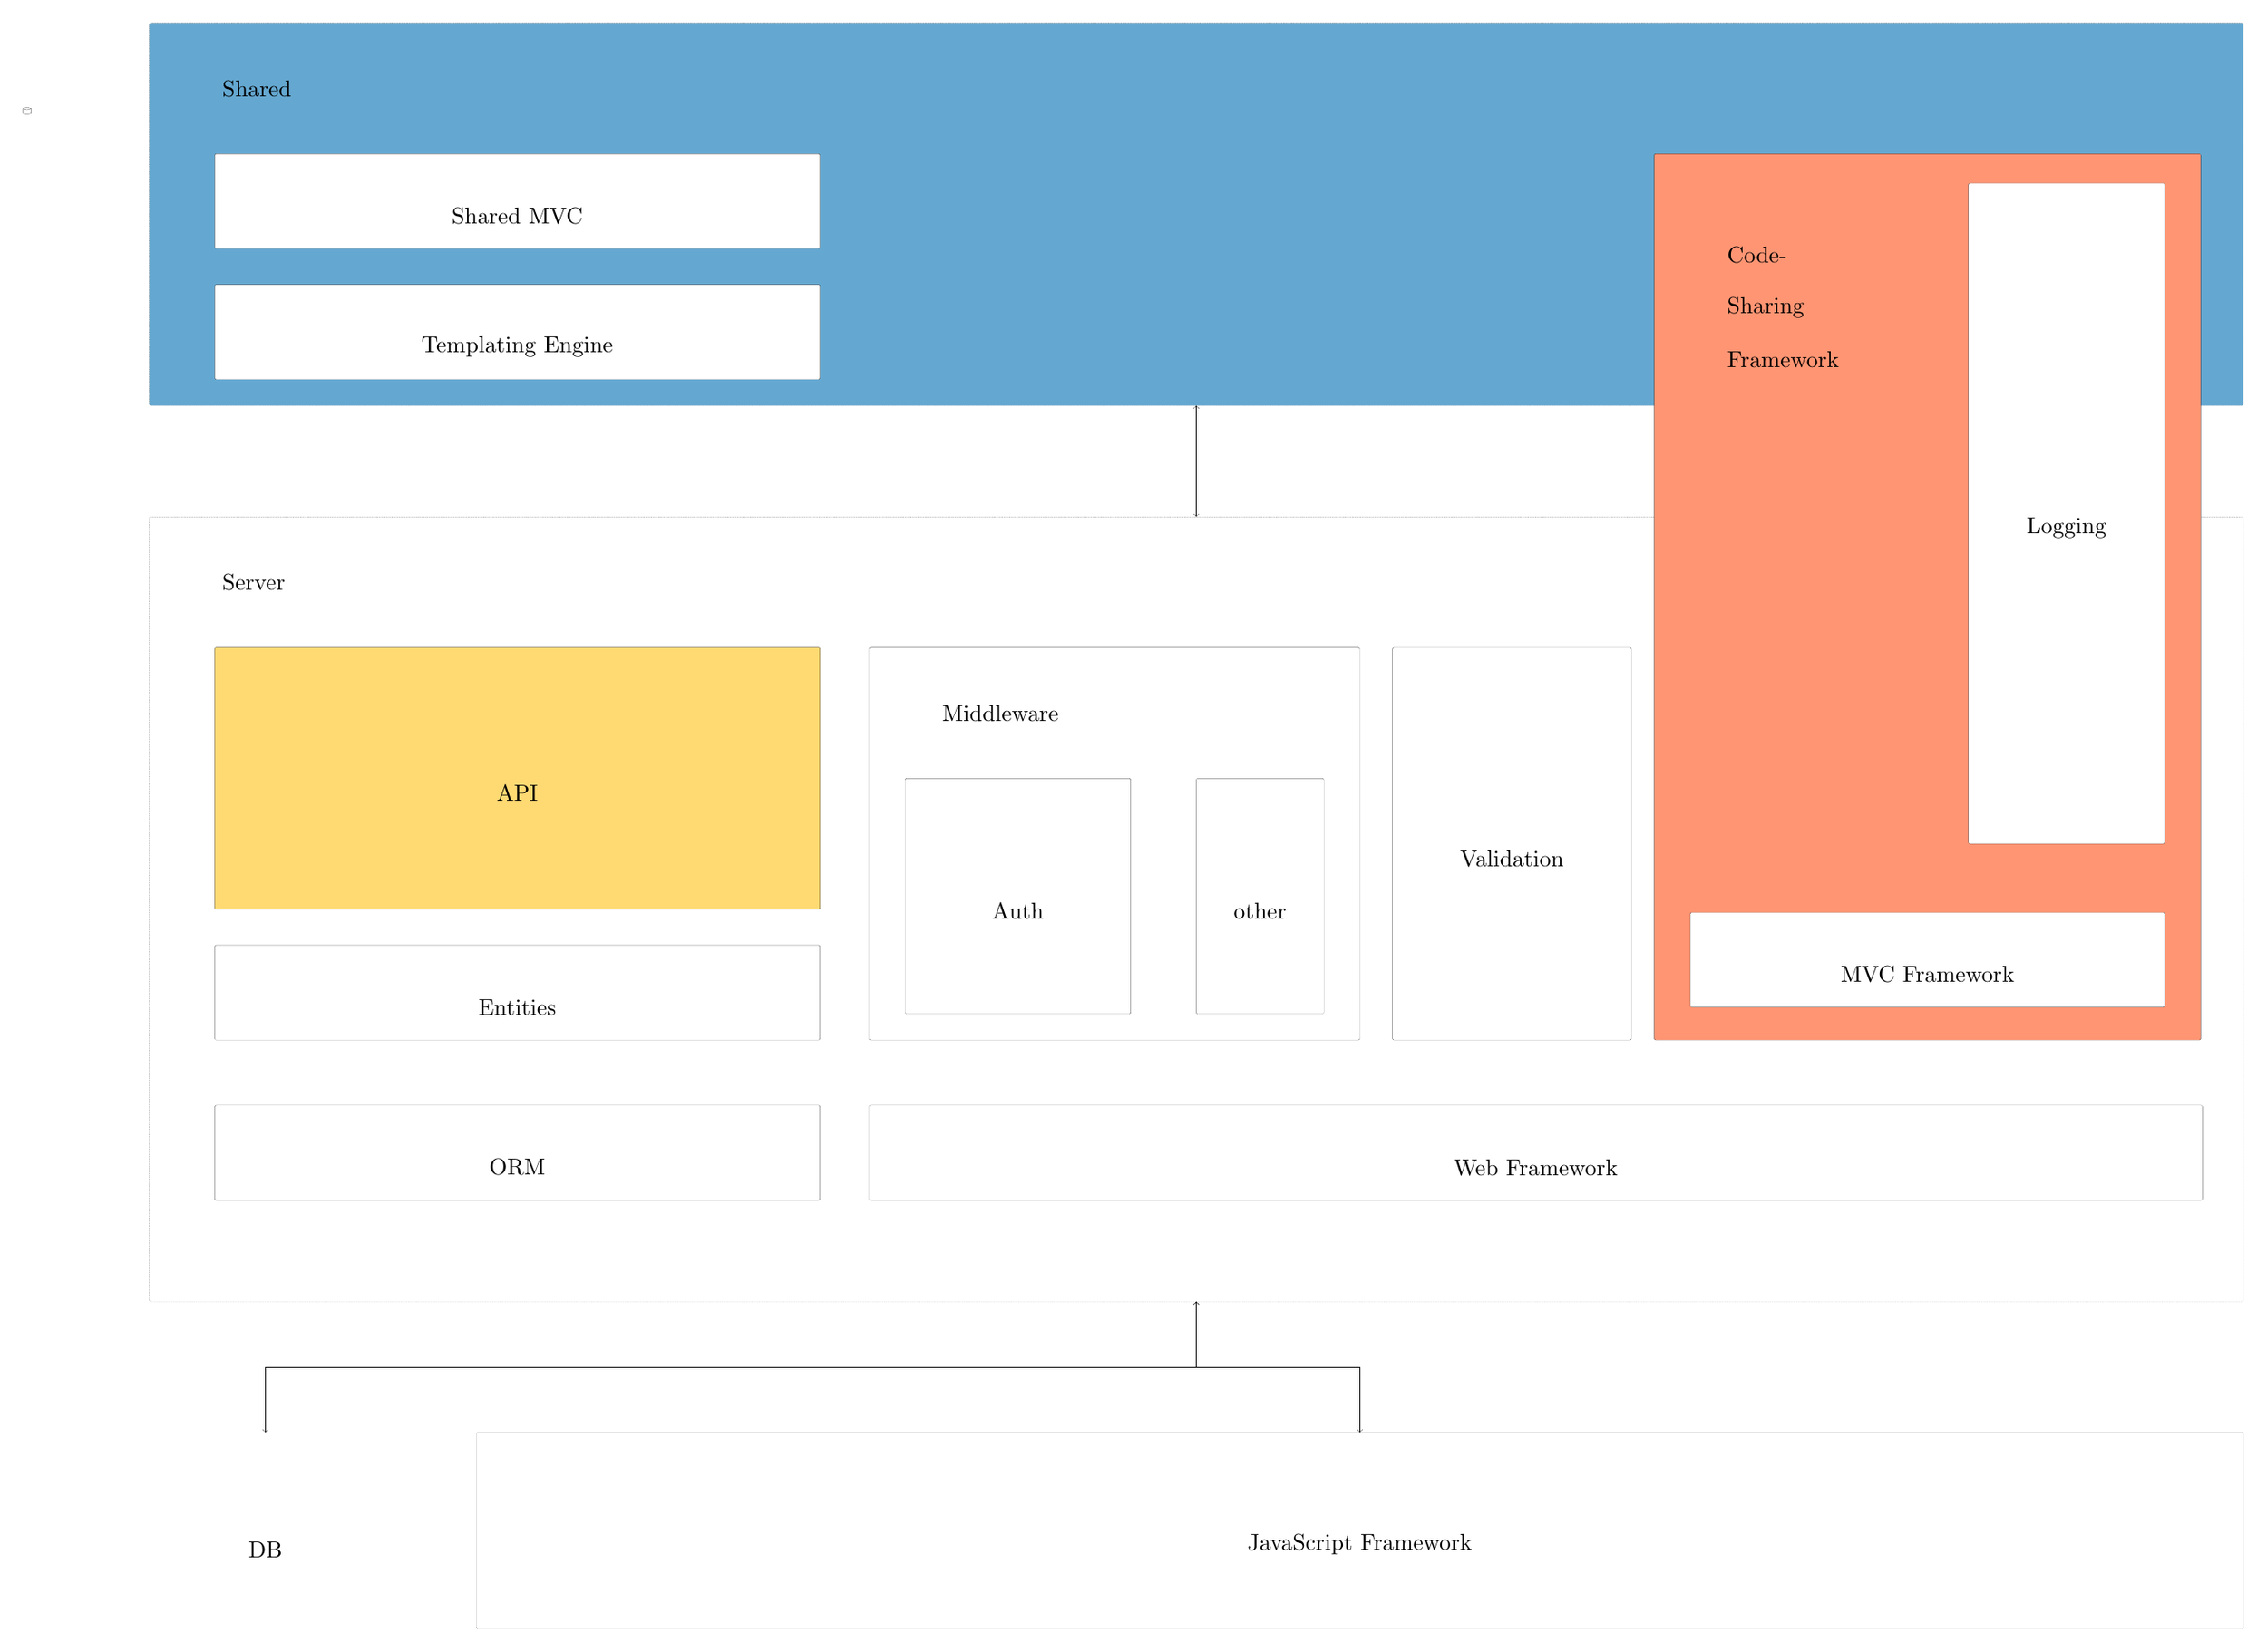
\begin{tikzpicture}
\pgftransformxscale{1.000000}
\pgftransformyscale{-1.000000}
\definecolor{dialinecolor}{rgb}{0.000000, 0.000000, 0.000000}
\pgfsetstrokecolor{dialinecolor}
\definecolor{dialinecolor}{rgb}{1.000000, 1.000000, 1.000000}
\pgfsetfillcolor{dialinecolor}
\pgfsetlinewidth{0.050000\du}
\pgfsetdash{{\pgflinewidth}{0.200000\du}}{0cm}
\pgfsetdash{{\pgflinewidth}{0.200000\du}}{0cm}
\pgfsetroundjoin
{\pgfsetcornersarced{\pgfpoint{0.500000\du}{0.500000\du}}\definecolor{dialinecolor}{rgb}{0.392157, 0.658824, 0.819608}
\pgfsetfillcolor{dialinecolor}
\fill (2.000000\du,-0.550000\du)--(2.000000\du,5.300000\du)--(34.000000\du,5.300000\du)--(34.000000\du,-0.550000\du)--cycle;
}{\pgfsetcornersarced{\pgfpoint{0.500000\du}{0.500000\du}}\definecolor{dialinecolor}{rgb}{0.000000, 0.000000, 0.000000}
\pgfsetstrokecolor{dialinecolor}
\draw (2.000000\du,-0.550000\du)--(2.000000\du,5.300000\du)--(34.000000\du,5.300000\du)--(34.000000\du,-0.550000\du)--cycle;
}% setfont left to latex
\definecolor{dialinecolor}{rgb}{0.000000, 0.000000, 0.000000}
\pgfsetstrokecolor{dialinecolor}
\node[anchor=west] at (3.000000\du,0.450000\du){Shared};
\pgfsetlinewidth{0.050000\du}
\pgfsetdash{{\pgflinewidth}{0.200000\du}}{0cm}
\pgfsetdash{{\pgflinewidth}{0.200000\du}}{0cm}
\pgfsetroundjoin
{\pgfsetcornersarced{\pgfpoint{0.500000\du}{0.500000\du}}\definecolor{dialinecolor}{rgb}{1.000000, 1.000000, 1.000000}
\pgfsetfillcolor{dialinecolor}
\fill (2.000000\du,7.000000\du)--(2.000000\du,19.000000\du)--(34.000000\du,19.000000\du)--(34.000000\du,7.000000\du)--cycle;
}{\pgfsetcornersarced{\pgfpoint{0.500000\du}{0.500000\du}}\definecolor{dialinecolor}{rgb}{0.000000, 0.000000, 0.000000}
\pgfsetstrokecolor{dialinecolor}
\draw (2.000000\du,7.000000\du)--(2.000000\du,19.000000\du)--(34.000000\du,19.000000\du)--(34.000000\du,7.000000\du)--cycle;
}\pgfsetlinewidth{0.050000\du}
\pgfsetdash{}{0pt}
\pgfsetdash{}{0pt}
\pgfsetbuttcap
\pgfsetmiterjoin
\pgfsetlinewidth{0.050000\du}
\pgfsetbuttcap
\pgfsetmiterjoin
\pgfsetdash{}{0pt}
\definecolor{dialinecolor}{rgb}{1.000000, 1.000000, 1.000000}
\pgfsetfillcolor{dialinecolor}
\pgfpathmoveto{\pgfpoint{2.000000\du}{21.525000\du}}
\pgfpathcurveto{\pgfpoint{2.710000\du}{21.131250\du}}{\pgfpoint{3.065000\du}{21.000000\du}}{\pgfpoint{3.775000\du}{21.000000\du}}
\pgfpathcurveto{\pgfpoint{4.485000\du}{21.000000\du}}{\pgfpoint{4.840000\du}{21.131250\du}}{\pgfpoint{5.550000\du}{21.525000\du}}
\pgfpathlineto{\pgfpoint{5.550000\du}{23.625000\du}}
\pgfpathcurveto{\pgfpoint{4.840000\du}{24.018750\du}}{\pgfpoint{4.485000\du}{24.150000\du}}{\pgfpoint{3.775000\du}{24.150000\du}}
\pgfpathcurveto{\pgfpoint{3.065000\du}{24.150000\du}}{\pgfpoint{2.710000\du}{24.018750\du}}{\pgfpoint{2.000000\du}{23.625000\du}}
\pgfpathlineto{\pgfpoint{2.000000\du}{21.525000\du}}
\pgfusepath{fill}
\definecolor{dialinecolor}{rgb}{0.000000, 0.000000, 0.000000}
\pgfsetstrokecolor{dialinecolor}
\pgfpathmoveto{\pgfpoint{2.000000\du}{21.525000\du}}
\pgfpathcurveto{\pgfpoint{2.710000\du}{21.131250\du}}{\pgfpoint{3.065000\du}{21.000000\du}}{\pgfpoint{3.775000\du}{21.000000\du}}
\pgfpathcurveto{\pgfpoint{4.485000\du}{21.000000\du}}{\pgfpoint{4.840000\du}{21.131250\du}}{\pgfpoint{5.550000\du}{21.525000\du}}
\pgfpathlineto{\pgfpoint{5.550000\du}{23.625000\du}}
\pgfpathcurveto{\pgfpoint{4.840000\du}{24.018750\du}}{\pgfpoint{4.485000\du}{24.150000\du}}{\pgfpoint{3.775000\du}{24.150000\du}}
\pgfpathcurveto{\pgfpoint{3.065000\du}{24.150000\du}}{\pgfpoint{2.710000\du}{24.018750\du}}{\pgfpoint{2.000000\du}{23.625000\du}}
\pgfpathlineto{\pgfpoint{2.000000\du}{21.525000\du}}
\pgfusepath{stroke}
\pgfsetbuttcap
\pgfsetmiterjoin
\pgfsetdash{}{0pt}
\definecolor{dialinecolor}{rgb}{0.000000, 0.000000, 0.000000}
\pgfsetstrokecolor{dialinecolor}
\pgfpathmoveto{\pgfpoint{2.000000\du}{21.525000\du}}
\pgfpathcurveto{\pgfpoint{2.710000\du}{21.918750\du}}{\pgfpoint{3.065000\du}{22.050000\du}}{\pgfpoint{3.775000\du}{22.050000\du}}
\pgfpathcurveto{\pgfpoint{4.485000\du}{22.050000\du}}{\pgfpoint{4.840000\du}{21.918750\du}}{\pgfpoint{5.550000\du}{21.525000\du}}
\pgfusepath{stroke}
% setfont left to latex
\definecolor{dialinecolor}{rgb}{0.000000, 0.000000, 0.000000}
\pgfsetstrokecolor{dialinecolor}
\node at (3.775000\du,23.037500\du){};
\pgfsetlinewidth{0.050000\du}
\pgfsetdash{}{0pt}
\pgfsetdash{}{0pt}
\pgfsetroundjoin
{\pgfsetcornersarced{\pgfpoint{0.500000\du}{0.500000\du}}\definecolor{dialinecolor}{rgb}{1.000000, 1.000000, 1.000000}
\pgfsetfillcolor{dialinecolor}
\fill (7.000000\du,21.000000\du)--(7.000000\du,24.000000\du)--(34.000000\du,24.000000\du)--(34.000000\du,21.000000\du)--cycle;
}{\pgfsetcornersarced{\pgfpoint{0.500000\du}{0.500000\du}}\definecolor{dialinecolor}{rgb}{0.000000, 0.000000, 0.000000}
\pgfsetstrokecolor{dialinecolor}
\draw (7.000000\du,21.000000\du)--(7.000000\du,24.000000\du)--(34.000000\du,24.000000\du)--(34.000000\du,21.000000\du)--cycle;
}% setfont left to latex
\definecolor{dialinecolor}{rgb}{0.000000, 0.000000, 0.000000}
\pgfsetstrokecolor{dialinecolor}
\node[anchor=west] at (3.000000\du,8.000000\du){Server};
\pgfsetlinewidth{0.050000\du}
\pgfsetdash{}{0pt}
\pgfsetdash{}{0pt}
\pgfsetroundjoin
{\pgfsetcornersarced{\pgfpoint{0.500000\du}{0.500000\du}}\definecolor{dialinecolor}{rgb}{1.000000, 0.854902, 0.450980}
\pgfsetfillcolor{dialinecolor}
\fill (3.000000\du,9.000000\du)--(3.000000\du,13.000000\du)--(12.250000\du,13.000000\du)--(12.250000\du,9.000000\du)--cycle;
}{\pgfsetcornersarced{\pgfpoint{0.500000\du}{0.500000\du}}\definecolor{dialinecolor}{rgb}{0.000000, 0.000000, 0.000000}
\pgfsetstrokecolor{dialinecolor}
\draw (3.000000\du,9.000000\du)--(3.000000\du,13.000000\du)--(12.250000\du,13.000000\du)--(12.250000\du,9.000000\du)--cycle;
}% setfont left to latex
\definecolor{dialinecolor}{rgb}{0.000000, 0.000000, 0.000000}
\pgfsetstrokecolor{dialinecolor}
\node at (7.625000\du,11.222500\du){API};
\pgfsetlinewidth{0.050000\du}
\pgfsetdash{}{0pt}
\pgfsetdash{}{0pt}
\pgfsetroundjoin
{\pgfsetcornersarced{\pgfpoint{0.500000\du}{0.500000\du}}\definecolor{dialinecolor}{rgb}{1.000000, 1.000000, 1.000000}
\pgfsetfillcolor{dialinecolor}
\fill (13.000000\du,9.000000\du)--(13.000000\du,15.000000\du)--(20.500000\du,15.000000\du)--(20.500000\du,9.000000\du)--cycle;
}{\pgfsetcornersarced{\pgfpoint{0.500000\du}{0.500000\du}}\definecolor{dialinecolor}{rgb}{0.000000, 0.000000, 0.000000}
\pgfsetstrokecolor{dialinecolor}
\draw (13.000000\du,9.000000\du)--(13.000000\du,15.000000\du)--(20.500000\du,15.000000\du)--(20.500000\du,9.000000\du)--cycle;
}% setfont left to latex
\definecolor{dialinecolor}{rgb}{0.000000, 0.000000, 0.000000}
\pgfsetstrokecolor{dialinecolor}
\node[anchor=west] at (14.000000\du,10.000000\du){Middleware};
\pgfsetlinewidth{0.050000\du}
\pgfsetdash{}{0pt}
\pgfsetdash{}{0pt}
\pgfsetroundjoin
{\pgfsetcornersarced{\pgfpoint{0.500000\du}{0.500000\du}}\definecolor{dialinecolor}{rgb}{1.000000, 0.584314, 0.450980}
\pgfsetfillcolor{dialinecolor}
\fill (25.000000\du,1.450000\du)--(25.000000\du,15.000000\du)--(33.350100\du,15.000000\du)--(33.350100\du,1.450000\du)--cycle;
}{\pgfsetcornersarced{\pgfpoint{0.500000\du}{0.500000\du}}\definecolor{dialinecolor}{rgb}{0.000000, 0.000000, 0.000000}
\pgfsetstrokecolor{dialinecolor}
\draw (25.000000\du,1.450000\du)--(25.000000\du,15.000000\du)--(33.350100\du,15.000000\du)--(33.350100\du,1.450000\du)--cycle;
}% setfont left to latex
\definecolor{dialinecolor}{rgb}{0.000000, 0.000000, 0.000000}
\pgfsetstrokecolor{dialinecolor}
\node[anchor=west] at (26.000000\du,3.000000\du){Code-};
% setfont left to latex
\definecolor{dialinecolor}{rgb}{0.000000, 0.000000, 0.000000}
\pgfsetstrokecolor{dialinecolor}
\node[anchor=west] at (26.000000\du,3.800000\du){Sharing};
% setfont left to latex
\definecolor{dialinecolor}{rgb}{0.000000, 0.000000, 0.000000}
\pgfsetstrokecolor{dialinecolor}
\node[anchor=west] at (26.000000\du,4.600000\du){Framework};
\pgfsetlinewidth{0.050000\du}
\pgfsetdash{}{0pt}
\pgfsetdash{}{0pt}
\pgfsetroundjoin
{\pgfsetcornersarced{\pgfpoint{0.500000\du}{0.500000\du}}\definecolor{dialinecolor}{rgb}{1.000000, 1.000000, 1.000000}
\pgfsetfillcolor{dialinecolor}
\fill (29.800000\du,1.900000\du)--(29.800000\du,12.000000\du)--(32.800000\du,12.000000\du)--(32.800000\du,1.900000\du)--cycle;
}{\pgfsetcornersarced{\pgfpoint{0.500000\du}{0.500000\du}}\definecolor{dialinecolor}{rgb}{0.000000, 0.000000, 0.000000}
\pgfsetstrokecolor{dialinecolor}
\draw (29.800000\du,1.900000\du)--(29.800000\du,12.000000\du)--(32.800000\du,12.000000\du)--(32.800000\du,1.900000\du)--cycle;
}% setfont left to latex
\definecolor{dialinecolor}{rgb}{0.000000, 0.000000, 0.000000}
\pgfsetstrokecolor{dialinecolor}
\node at (31.300000\du,7.172500\du){Logging};
\pgfsetlinewidth{0.050000\du}
\pgfsetdash{}{0pt}
\pgfsetdash{}{0pt}
\pgfsetroundjoin
{\pgfsetcornersarced{\pgfpoint{0.500000\du}{0.500000\du}}\definecolor{dialinecolor}{rgb}{1.000000, 1.000000, 1.000000}
\pgfsetfillcolor{dialinecolor}
\fill (13.550000\du,11.000000\du)--(13.550000\du,14.600000\du)--(17.000000\du,14.600000\du)--(17.000000\du,11.000000\du)--cycle;
}{\pgfsetcornersarced{\pgfpoint{0.500000\du}{0.500000\du}}\definecolor{dialinecolor}{rgb}{0.000000, 0.000000, 0.000000}
\pgfsetstrokecolor{dialinecolor}
\draw (13.550000\du,11.000000\du)--(13.550000\du,14.600000\du)--(17.000000\du,14.600000\du)--(17.000000\du,11.000000\du)--cycle;
}% setfont left to latex
\definecolor{dialinecolor}{rgb}{0.000000, 0.000000, 0.000000}
\pgfsetstrokecolor{dialinecolor}
\node at (15.275000\du,13.022500\du){Auth};
\pgfsetlinewidth{0.050000\du}
\pgfsetdash{}{0pt}
\pgfsetdash{}{0pt}
\pgfsetroundjoin
{\pgfsetcornersarced{\pgfpoint{0.500000\du}{0.500000\du}}\definecolor{dialinecolor}{rgb}{1.000000, 1.000000, 1.000000}
\pgfsetfillcolor{dialinecolor}
\fill (21.000000\du,8.998940\du)--(21.000000\du,15.000003\du)--(24.650000\du,15.000003\du)--(24.650000\du,8.998940\du)--cycle;
}{\pgfsetcornersarced{\pgfpoint{0.500000\du}{0.500000\du}}\definecolor{dialinecolor}{rgb}{0.000000, 0.000000, 0.000000}
\pgfsetstrokecolor{dialinecolor}
\draw (21.000000\du,8.998940\du)--(21.000000\du,15.000003\du)--(24.650000\du,15.000003\du)--(24.650000\du,8.998940\du)--cycle;
}% setfont left to latex
\definecolor{dialinecolor}{rgb}{0.000000, 0.000000, 0.000000}
\pgfsetstrokecolor{dialinecolor}
\node at (22.825000\du,12.222000\du){Validation};
\pgfsetlinewidth{0.050000\du}
\pgfsetdash{}{0pt}
\pgfsetdash{}{0pt}
\pgfsetroundjoin
{\pgfsetcornersarced{\pgfpoint{0.500000\du}{0.500000\du}}\definecolor{dialinecolor}{rgb}{1.000000, 1.000000, 1.000000}
\pgfsetfillcolor{dialinecolor}
\fill (3.000000\du,13.550000\du)--(3.000000\du,15.000000\du)--(12.250000\du,15.000000\du)--(12.250000\du,13.550000\du)--cycle;
}{\pgfsetcornersarced{\pgfpoint{0.500000\du}{0.500000\du}}\definecolor{dialinecolor}{rgb}{0.000000, 0.000000, 0.000000}
\pgfsetstrokecolor{dialinecolor}
\draw (3.000000\du,13.550000\du)--(3.000000\du,15.000000\du)--(12.250000\du,15.000000\du)--(12.250000\du,13.550000\du)--cycle;
}% setfont left to latex
\definecolor{dialinecolor}{rgb}{0.000000, 0.000000, 0.000000}
\pgfsetstrokecolor{dialinecolor}
\node at (7.625000\du,14.497500\du){Entities};
% setfont left to latex
\definecolor{dialinecolor}{rgb}{0.000000, 0.000000, 0.000000}
\pgfsetstrokecolor{dialinecolor}
\node at (20.500000\du,22.713187\du){JavaScript Framework};
% setfont left to latex
\definecolor{dialinecolor}{rgb}{0.000000, 0.000000, 0.000000}
\pgfsetstrokecolor{dialinecolor}
\node at (3.775000\du,22.797500\du){DB};
% setfont left to latex
\definecolor{dialinecolor}{rgb}{0.000000, 0.000000, 0.000000}
\pgfsetstrokecolor{dialinecolor}
\node[anchor=west] at (7.625000\du,3.000000\du){};
\pgfsetlinewidth{0.050000\du}
\pgfsetdash{}{0pt}
\pgfsetdash{}{0pt}
\pgfsetroundjoin
{\pgfsetcornersarced{\pgfpoint{0.500000\du}{0.500000\du}}\definecolor{dialinecolor}{rgb}{1.000000, 1.000000, 1.000000}
\pgfsetfillcolor{dialinecolor}
\fill (18.000000\du,11.000000\du)--(18.000000\du,14.600000\du)--(19.950000\du,14.600000\du)--(19.950000\du,11.000000\du)--cycle;
}{\pgfsetcornersarced{\pgfpoint{0.500000\du}{0.500000\du}}\definecolor{dialinecolor}{rgb}{0.000000, 0.000000, 0.000000}
\pgfsetstrokecolor{dialinecolor}
\draw (18.000000\du,11.000000\du)--(18.000000\du,14.600000\du)--(19.950000\du,14.600000\du)--(19.950000\du,11.000000\du)--cycle;
}% setfont left to latex
\definecolor{dialinecolor}{rgb}{0.000000, 0.000000, 0.000000}
\pgfsetstrokecolor{dialinecolor}
\node at (18.975000\du,13.022500\du){other};
\pgfsetlinewidth{0.050000\du}
\pgfsetdash{}{0pt}
\pgfsetdash{}{0pt}
\pgfsetroundjoin
{\pgfsetcornersarced{\pgfpoint{0.500000\du}{0.500000\du}}\definecolor{dialinecolor}{rgb}{1.000000, 1.000000, 1.000000}
\pgfsetfillcolor{dialinecolor}
\fill (3.000000\du,1.450000\du)--(3.000000\du,2.900000\du)--(12.250000\du,2.900000\du)--(12.250000\du,1.450000\du)--cycle;
}{\pgfsetcornersarced{\pgfpoint{0.500000\du}{0.500000\du}}\definecolor{dialinecolor}{rgb}{0.000000, 0.000000, 0.000000}
\pgfsetstrokecolor{dialinecolor}
\draw (3.000000\du,1.450000\du)--(3.000000\du,2.900000\du)--(12.250000\du,2.900000\du)--(12.250000\du,1.450000\du)--cycle;
}\pgfsetlinewidth{0.050000\du}
\pgfsetdash{}{0pt}
\pgfsetdash{}{0pt}
\pgfsetroundjoin
{\pgfsetcornersarced{\pgfpoint{0.500000\du}{0.500000\du}}\definecolor{dialinecolor}{rgb}{1.000000, 1.000000, 1.000000}
\pgfsetfillcolor{dialinecolor}
\fill (25.550000\du,13.050000\du)--(25.550000\du,14.500000\du)--(32.800000\du,14.500000\du)--(32.800000\du,13.050000\du)--cycle;
}{\pgfsetcornersarced{\pgfpoint{0.500000\du}{0.500000\du}}\definecolor{dialinecolor}{rgb}{0.000000, 0.000000, 0.000000}
\pgfsetstrokecolor{dialinecolor}
\draw (25.550000\du,13.050000\du)--(25.550000\du,14.500000\du)--(32.800000\du,14.500000\du)--(32.800000\du,13.050000\du)--cycle;
}\pgfsetlinewidth{0.050000\du}
\pgfsetdash{}{0pt}
\pgfsetdash{}{0pt}
\pgfsetroundjoin
{\pgfsetcornersarced{\pgfpoint{0.500000\du}{0.500000\du}}\definecolor{dialinecolor}{rgb}{1.000000, 1.000000, 1.000000}
\pgfsetfillcolor{dialinecolor}
\fill (13.000000\du,16.000000\du)--(13.000000\du,17.450000\du)--(33.375000\du,17.450000\du)--(33.375000\du,16.000000\du)--cycle;
}{\pgfsetcornersarced{\pgfpoint{0.500000\du}{0.500000\du}}\definecolor{dialinecolor}{rgb}{0.000000, 0.000000, 0.000000}
\pgfsetstrokecolor{dialinecolor}
\draw (13.000000\du,16.000000\du)--(13.000000\du,17.450000\du)--(33.375000\du,17.450000\du)--(33.375000\du,16.000000\du)--cycle;
}\pgfsetlinewidth{0.050000\du}
\pgfsetdash{}{0pt}
\pgfsetdash{}{0pt}
\pgfsetroundjoin
{\pgfsetcornersarced{\pgfpoint{0.500000\du}{0.500000\du}}\definecolor{dialinecolor}{rgb}{1.000000, 1.000000, 1.000000}
\pgfsetfillcolor{dialinecolor}
\fill (3.000000\du,16.000000\du)--(3.000000\du,17.450000\du)--(12.250000\du,17.450000\du)--(12.250000\du,16.000000\du)--cycle;
}{\pgfsetcornersarced{\pgfpoint{0.500000\du}{0.500000\du}}\definecolor{dialinecolor}{rgb}{0.000000, 0.000000, 0.000000}
\pgfsetstrokecolor{dialinecolor}
\draw (3.000000\du,16.000000\du)--(3.000000\du,17.450000\du)--(12.250000\du,17.450000\du)--(12.250000\du,16.000000\du)--cycle;
}\pgfsetlinewidth{0.050000\du}
\pgfsetdash{}{0pt}
\pgfsetdash{}{0pt}
\pgfsetroundjoin
{\pgfsetcornersarced{\pgfpoint{0.500000\du}{0.500000\du}}\definecolor{dialinecolor}{rgb}{1.000000, 1.000000, 1.000000}
\pgfsetfillcolor{dialinecolor}
\fill (3.000000\du,3.450000\du)--(3.000000\du,4.900000\du)--(12.250000\du,4.900000\du)--(12.250000\du,3.450000\du)--cycle;
}{\pgfsetcornersarced{\pgfpoint{0.500000\du}{0.500000\du}}\definecolor{dialinecolor}{rgb}{0.000000, 0.000000, 0.000000}
\pgfsetstrokecolor{dialinecolor}
\draw (3.000000\du,3.450000\du)--(3.000000\du,4.900000\du)--(12.250000\du,4.900000\du)--(12.250000\du,3.450000\du)--cycle;
}% setfont left to latex
\definecolor{dialinecolor}{rgb}{0.000000, 0.000000, 0.000000}
\pgfsetstrokecolor{dialinecolor}
\node at (7.625000\du,2.397500\du){Shared MVC};
% setfont left to latex
\definecolor{dialinecolor}{rgb}{0.000000, 0.000000, 0.000000}
\pgfsetstrokecolor{dialinecolor}
\node at (7.625000\du,4.397500\du){Templating Engine};
% setfont left to latex
\definecolor{dialinecolor}{rgb}{0.000000, 0.000000, 0.000000}
\pgfsetstrokecolor{dialinecolor}
\node at (29.175000\du,13.997500\du){MVC Framework};
% setfont left to latex
\definecolor{dialinecolor}{rgb}{0.000000, 0.000000, 0.000000}
\pgfsetstrokecolor{dialinecolor}
\node at (7.625000\du,16.947500\du){ORM};
% setfont left to latex
\definecolor{dialinecolor}{rgb}{0.000000, 0.000000, 0.000000}
\pgfsetstrokecolor{dialinecolor}
\node at (23.187500\du,16.947500\du){Web Framework};
\pgfsetlinewidth{0.100000\du}
\pgfsetdash{}{0pt}
\pgfsetdash{}{0pt}
\pgfsetmiterjoin
\pgfsetbuttcap
{
\definecolor{dialinecolor}{rgb}{0.000000, 0.000000, 0.000000}
\pgfsetfillcolor{dialinecolor}
% was here!!!
\pgfsetarrowsstart{to}
\pgfsetarrowsend{to}
{\pgfsetcornersarced{\pgfpoint{0.000000\du}{0.000000\du}}\definecolor{dialinecolor}{rgb}{0.000000, 0.000000, 0.000000}
\pgfsetstrokecolor{dialinecolor}
\draw (20.500000\du,21.000000\du)--(20.500000\du,20.000000\du)--(18.000000\du,20.000000\du)--(18.000000\du,19.000000\du);
}}
\pgfsetlinewidth{0.100000\du}
\pgfsetdash{}{0pt}
\pgfsetdash{}{0pt}
\pgfsetmiterjoin
\pgfsetbuttcap
{
\definecolor{dialinecolor}{rgb}{0.000000, 0.000000, 0.000000}
\pgfsetfillcolor{dialinecolor}
% was here!!!
\pgfsetarrowsstart{to}
\pgfsetarrowsend{to}
{\pgfsetcornersarced{\pgfpoint{0.000000\du}{0.000000\du}}\definecolor{dialinecolor}{rgb}{0.000000, 0.000000, 0.000000}
\pgfsetstrokecolor{dialinecolor}
\draw (3.775000\du,21.000000\du)--(3.775000\du,20.000000\du)--(18.000000\du,20.000000\du)--(18.000000\du,19.000000\du);
}}
\pgfsetlinewidth{0.100000\du}
\pgfsetdash{}{0pt}
\pgfsetdash{}{0pt}
\pgfsetbuttcap
{
\definecolor{dialinecolor}{rgb}{0.000000, 0.000000, 0.000000}
\pgfsetfillcolor{dialinecolor}
% was here!!!
\pgfsetarrowsstart{to}
\pgfsetarrowsend{to}
\definecolor{dialinecolor}{rgb}{0.000000, 0.000000, 0.000000}
\pgfsetstrokecolor{dialinecolor}
\draw (18.000000\du,7.000000\du)--(18.000000\du,5.300000\du);
}
\end{tikzpicture}

	}

	\caption{Software Layers -- Technologieneutral}
\end{figure}

\subsubsection*{Shared}
Die ``Shared''-Schicht beinhaltet jeglicher Quelltext, welcher sowohl auf Client als auch auf Server-Seite instanziert wird.

\subsubsection*{Shared MVC}
Jeglicher Quelltext auf der ``Shared''-Schicht ist mithilfe des MVC-Patterns strukturiert.

\subsubsection*{Templating Engine}
Das rendern der Views wird mithilfe einer Templating Engine vereinfacht.

\subsubsection*{API}
Es existiert eine entkoppelte \gls{REST}-API, welche von der ``Shared MVC''-Schicht für das manipulieren von Daten verwendet wird.

\subsubsection*{Entities}
Als Entities werden die \gls{ORM}-Models bezeichnet, welche Datenbanktabellen abstrahieren und die manipulation derer ermöglichen.

\subsubsection*{ORM}
Das ORM abstrahiert die Datenkbank-Verbindung und die Interaktion mit der Datenbank.

\subsubsection*{\gls{Middleware}}
Die \gls{Middleware} ist ein Konzept des verwendeten ``Web Frameworks'' und ermöglicht das manipulieren der ``Request'' und ``Response''.
Die Middleware-Schicht beinhaltet mehrere Middlewares und nur eine davon ist ``Auth''.

\subsubsection*{Auth}
Auth ist eine speziell hervorgehobene Middleware, welche die Authentifizierung von Besuchern ermöglicht.

\subsubsection*{Web Framework}
Das Web Framework stellt Funktionen zur Verfügung, um ``Request'' und ``Response'' einfacher verarbeiten zu können.

\subsubsection*{Validation}
Die Validations-Schicht besteht aus mehreren Validatoren, welche die datenbasierte Validierung übernehmen. Datenbasierte Validierung bedeutet, dass die vom Client gesendeten Daten bezüglich dem Datentyp überprüft werden.

\subsubsection*{Code Sharing Framework}
Während der Bachelorarbeit wurde ein sogenanntes ``Code Sharing Framework'' entwickelt, welches die Architektur ermöglicht hat. Es erlaubt das instanzieren des gleichen Quelltexts auf Server- wie auch auf Client-Seite.

\subsubsection*{Logging}
Das Code Sharing Framework loggt jeden Request und mögliche Fehler mithilfe einer Logging-Komponente.

\subsubsection*{MVC Framework}
Das MVC Framework wird vom Code Sharing Framework verwendet, und bietet Basisklassen dafür.

\subsection*{Konkrete Implementation}

\begin{figure}[H]
	\centering{
		% Graphic for TeX using PGF
% Title: dokumentation/content/sad/diagrams/layers-diagram-impl.dia
% Creator: Dia v0.97.2
% CreationDate: Wed Jun 12 08:00:26 2013
% For: michael
% \usepackage{tikz}
% The following commands are not supported in PSTricks at present
% We define them conditionally, so when they are implemented,
% this pgf file will use them.
\ifx\du\undefined
  \newlength{\du}
\fi
\setlength{\du}{13\unitlength}
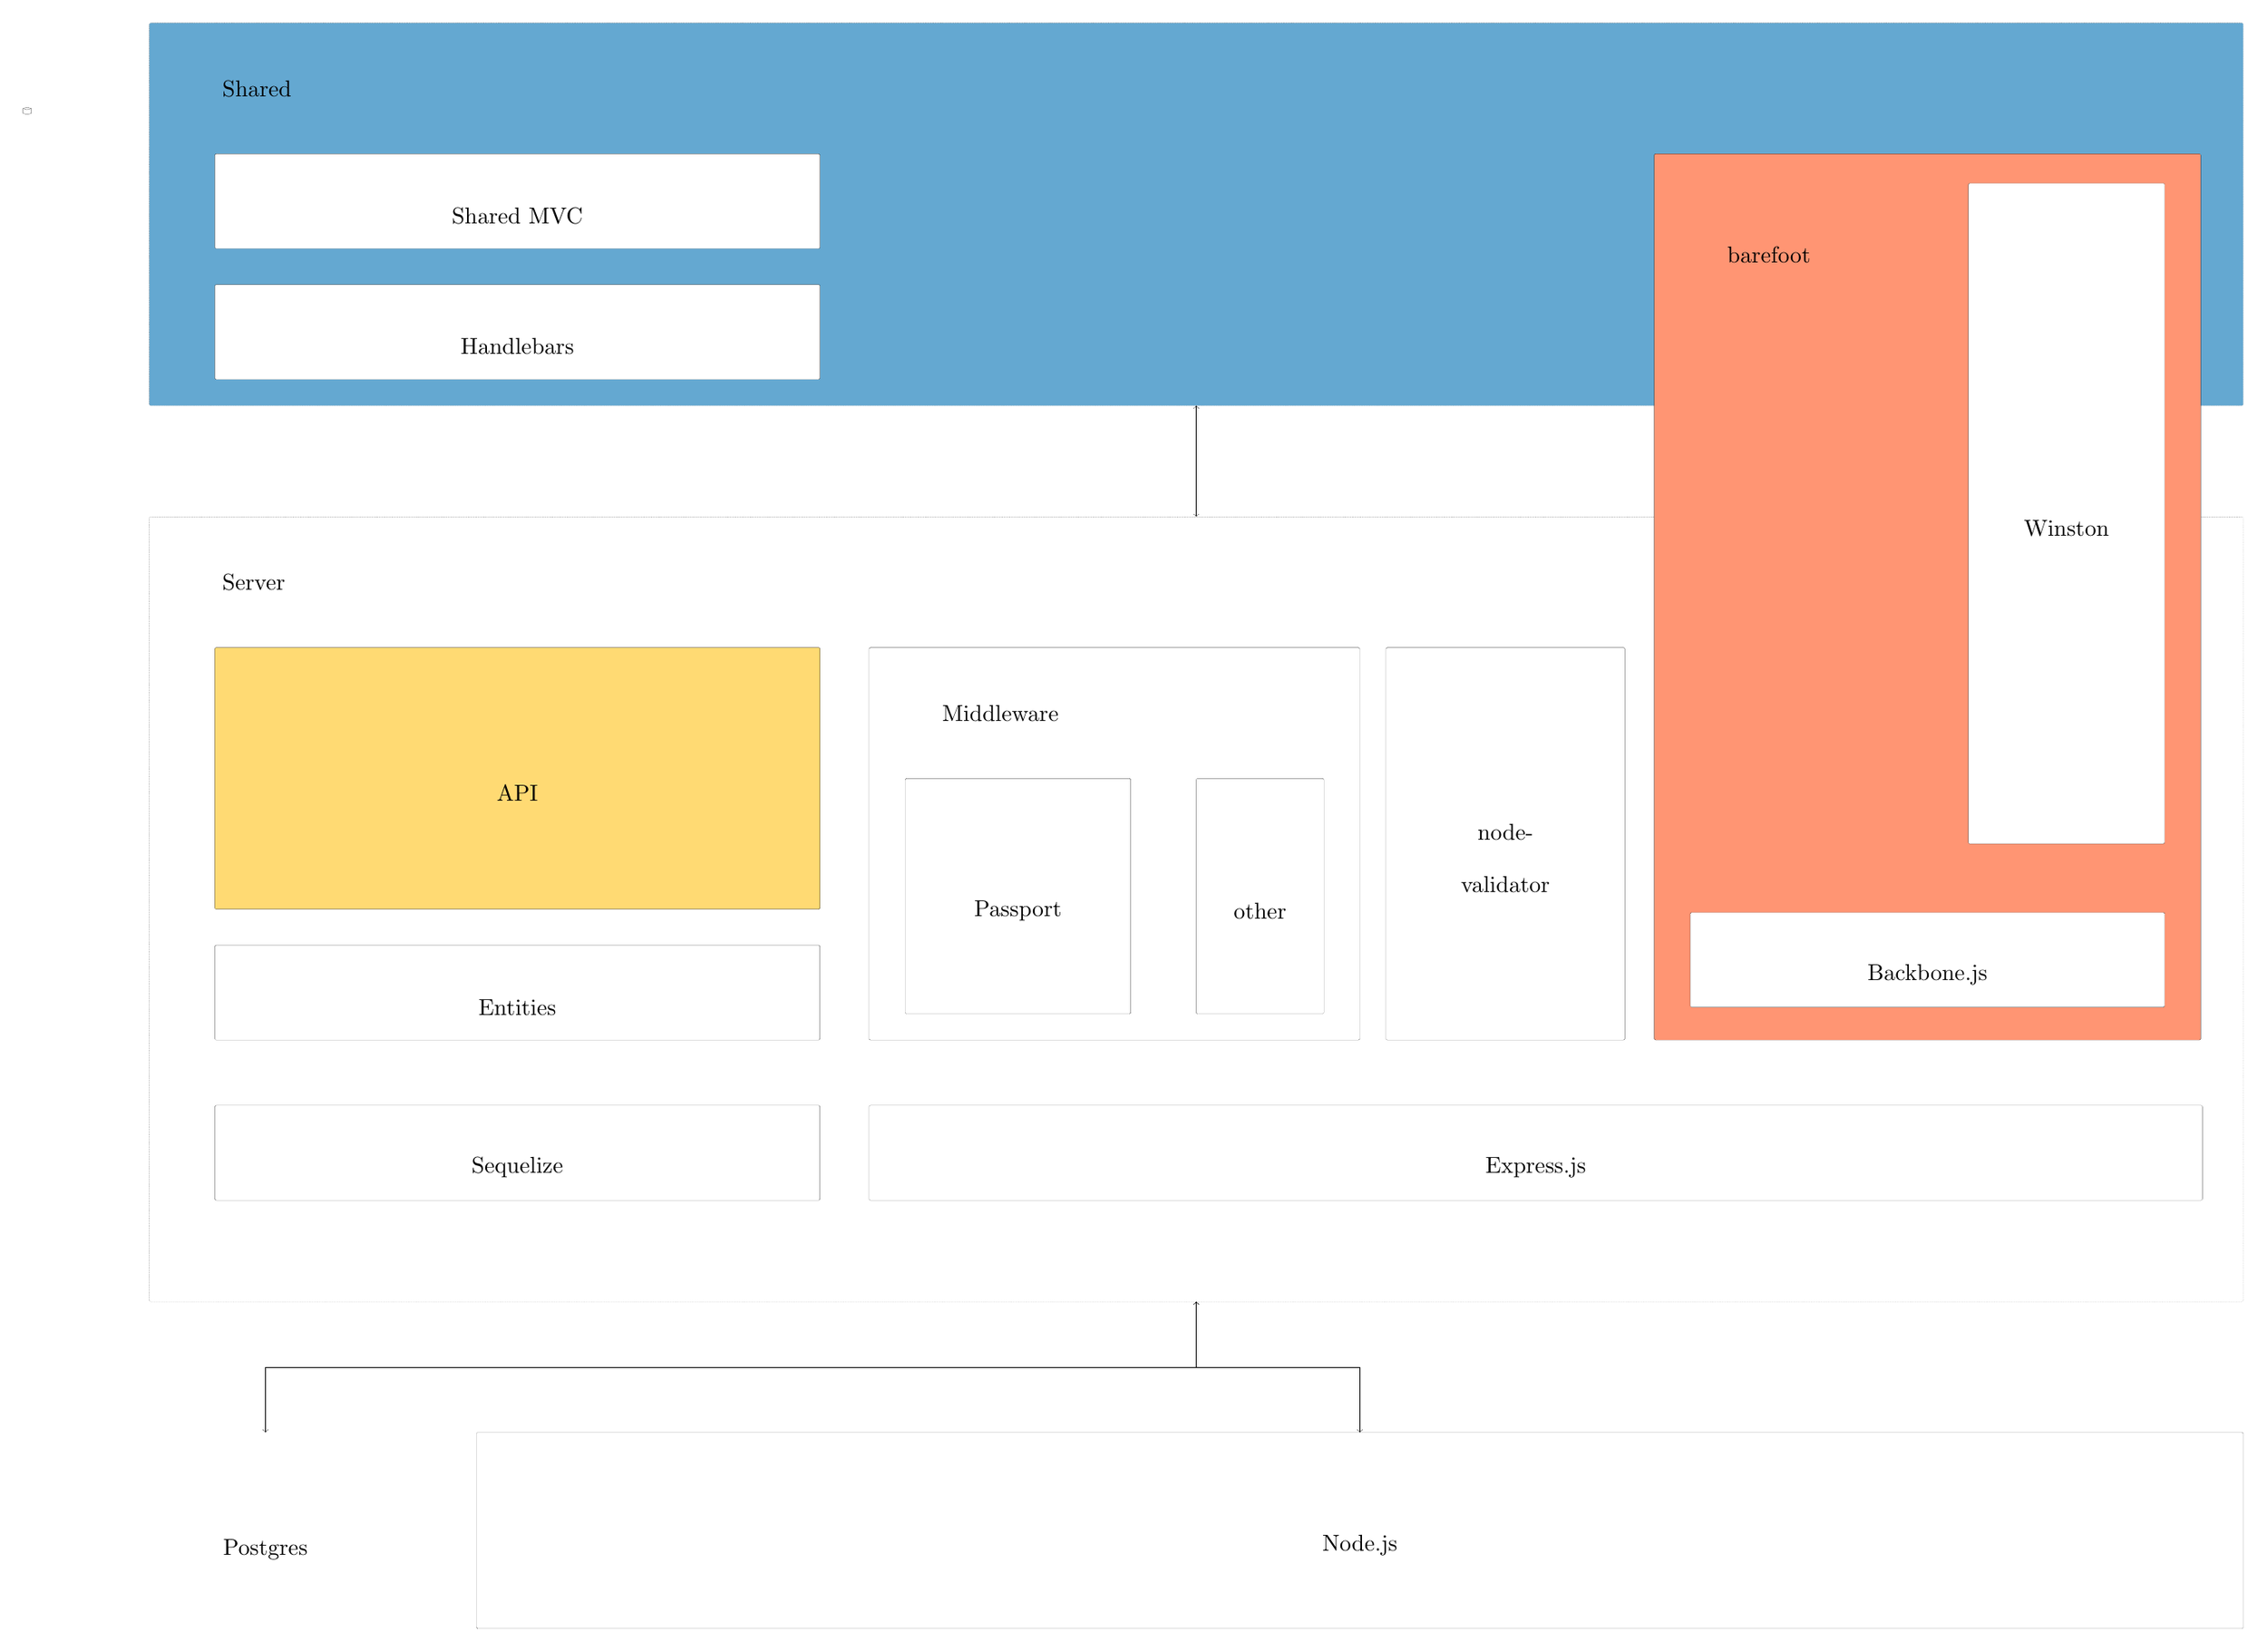
\begin{tikzpicture}
\pgftransformxscale{1.000000}
\pgftransformyscale{-1.000000}
\definecolor{dialinecolor}{rgb}{0.000000, 0.000000, 0.000000}
\pgfsetstrokecolor{dialinecolor}
\definecolor{dialinecolor}{rgb}{1.000000, 1.000000, 1.000000}
\pgfsetfillcolor{dialinecolor}
\pgfsetlinewidth{0.050000\du}
\pgfsetdash{{\pgflinewidth}{0.200000\du}}{0cm}
\pgfsetdash{{\pgflinewidth}{0.200000\du}}{0cm}
\pgfsetroundjoin
{\pgfsetcornersarced{\pgfpoint{0.500000\du}{0.500000\du}}\definecolor{dialinecolor}{rgb}{0.392157, 0.658824, 0.819608}
\pgfsetfillcolor{dialinecolor}
\fill (2.000000\du,-0.550000\du)--(2.000000\du,5.300000\du)--(34.000000\du,5.300000\du)--(34.000000\du,-0.550000\du)--cycle;
}{\pgfsetcornersarced{\pgfpoint{0.500000\du}{0.500000\du}}\definecolor{dialinecolor}{rgb}{0.000000, 0.000000, 0.000000}
\pgfsetstrokecolor{dialinecolor}
\draw (2.000000\du,-0.550000\du)--(2.000000\du,5.300000\du)--(34.000000\du,5.300000\du)--(34.000000\du,-0.550000\du)--cycle;
}% setfont left to latex
\definecolor{dialinecolor}{rgb}{0.000000, 0.000000, 0.000000}
\pgfsetstrokecolor{dialinecolor}
\node[anchor=west] at (3.000000\du,0.450000\du){Shared};
\pgfsetlinewidth{0.050000\du}
\pgfsetdash{{\pgflinewidth}{0.200000\du}}{0cm}
\pgfsetdash{{\pgflinewidth}{0.200000\du}}{0cm}
\pgfsetroundjoin
{\pgfsetcornersarced{\pgfpoint{0.500000\du}{0.500000\du}}\definecolor{dialinecolor}{rgb}{1.000000, 1.000000, 1.000000}
\pgfsetfillcolor{dialinecolor}
\fill (2.000000\du,7.000000\du)--(2.000000\du,19.000000\du)--(34.000000\du,19.000000\du)--(34.000000\du,7.000000\du)--cycle;
}{\pgfsetcornersarced{\pgfpoint{0.500000\du}{0.500000\du}}\definecolor{dialinecolor}{rgb}{0.000000, 0.000000, 0.000000}
\pgfsetstrokecolor{dialinecolor}
\draw (2.000000\du,7.000000\du)--(2.000000\du,19.000000\du)--(34.000000\du,19.000000\du)--(34.000000\du,7.000000\du)--cycle;
}\pgfsetlinewidth{0.050000\du}
\pgfsetdash{}{0pt}
\pgfsetdash{}{0pt}
\pgfsetbuttcap
\pgfsetmiterjoin
\pgfsetlinewidth{0.050000\du}
\pgfsetbuttcap
\pgfsetmiterjoin
\pgfsetdash{}{0pt}
\definecolor{dialinecolor}{rgb}{1.000000, 1.000000, 1.000000}
\pgfsetfillcolor{dialinecolor}
\pgfpathmoveto{\pgfpoint{2.000000\du}{21.525000\du}}
\pgfpathcurveto{\pgfpoint{2.710000\du}{21.131250\du}}{\pgfpoint{3.065000\du}{21.000000\du}}{\pgfpoint{3.775000\du}{21.000000\du}}
\pgfpathcurveto{\pgfpoint{4.485000\du}{21.000000\du}}{\pgfpoint{4.840000\du}{21.131250\du}}{\pgfpoint{5.550000\du}{21.525000\du}}
\pgfpathlineto{\pgfpoint{5.550000\du}{23.625000\du}}
\pgfpathcurveto{\pgfpoint{4.840000\du}{24.018750\du}}{\pgfpoint{4.485000\du}{24.150000\du}}{\pgfpoint{3.775000\du}{24.150000\du}}
\pgfpathcurveto{\pgfpoint{3.065000\du}{24.150000\du}}{\pgfpoint{2.710000\du}{24.018750\du}}{\pgfpoint{2.000000\du}{23.625000\du}}
\pgfpathlineto{\pgfpoint{2.000000\du}{21.525000\du}}
\pgfusepath{fill}
\definecolor{dialinecolor}{rgb}{0.000000, 0.000000, 0.000000}
\pgfsetstrokecolor{dialinecolor}
\pgfpathmoveto{\pgfpoint{2.000000\du}{21.525000\du}}
\pgfpathcurveto{\pgfpoint{2.710000\du}{21.131250\du}}{\pgfpoint{3.065000\du}{21.000000\du}}{\pgfpoint{3.775000\du}{21.000000\du}}
\pgfpathcurveto{\pgfpoint{4.485000\du}{21.000000\du}}{\pgfpoint{4.840000\du}{21.131250\du}}{\pgfpoint{5.550000\du}{21.525000\du}}
\pgfpathlineto{\pgfpoint{5.550000\du}{23.625000\du}}
\pgfpathcurveto{\pgfpoint{4.840000\du}{24.018750\du}}{\pgfpoint{4.485000\du}{24.150000\du}}{\pgfpoint{3.775000\du}{24.150000\du}}
\pgfpathcurveto{\pgfpoint{3.065000\du}{24.150000\du}}{\pgfpoint{2.710000\du}{24.018750\du}}{\pgfpoint{2.000000\du}{23.625000\du}}
\pgfpathlineto{\pgfpoint{2.000000\du}{21.525000\du}}
\pgfusepath{stroke}
\pgfsetbuttcap
\pgfsetmiterjoin
\pgfsetdash{}{0pt}
\definecolor{dialinecolor}{rgb}{0.000000, 0.000000, 0.000000}
\pgfsetstrokecolor{dialinecolor}
\pgfpathmoveto{\pgfpoint{2.000000\du}{21.525000\du}}
\pgfpathcurveto{\pgfpoint{2.710000\du}{21.918750\du}}{\pgfpoint{3.065000\du}{22.050000\du}}{\pgfpoint{3.775000\du}{22.050000\du}}
\pgfpathcurveto{\pgfpoint{4.485000\du}{22.050000\du}}{\pgfpoint{4.840000\du}{21.918750\du}}{\pgfpoint{5.550000\du}{21.525000\du}}
\pgfusepath{stroke}
% setfont left to latex
\definecolor{dialinecolor}{rgb}{0.000000, 0.000000, 0.000000}
\pgfsetstrokecolor{dialinecolor}
\node at (3.775000\du,23.037500\du){};
\pgfsetlinewidth{0.050000\du}
\pgfsetdash{}{0pt}
\pgfsetdash{}{0pt}
\pgfsetroundjoin
{\pgfsetcornersarced{\pgfpoint{0.500000\du}{0.500000\du}}\definecolor{dialinecolor}{rgb}{1.000000, 1.000000, 1.000000}
\pgfsetfillcolor{dialinecolor}
\fill (7.000000\du,21.000000\du)--(7.000000\du,24.000000\du)--(34.000000\du,24.000000\du)--(34.000000\du,21.000000\du)--cycle;
}{\pgfsetcornersarced{\pgfpoint{0.500000\du}{0.500000\du}}\definecolor{dialinecolor}{rgb}{0.000000, 0.000000, 0.000000}
\pgfsetstrokecolor{dialinecolor}
\draw (7.000000\du,21.000000\du)--(7.000000\du,24.000000\du)--(34.000000\du,24.000000\du)--(34.000000\du,21.000000\du)--cycle;
}% setfont left to latex
\definecolor{dialinecolor}{rgb}{0.000000, 0.000000, 0.000000}
\pgfsetstrokecolor{dialinecolor}
\node[anchor=west] at (3.000000\du,8.000000\du){Server};
\pgfsetlinewidth{0.050000\du}
\pgfsetdash{}{0pt}
\pgfsetdash{}{0pt}
\pgfsetroundjoin
{\pgfsetcornersarced{\pgfpoint{0.500000\du}{0.500000\du}}\definecolor{dialinecolor}{rgb}{1.000000, 0.854902, 0.450980}
\pgfsetfillcolor{dialinecolor}
\fill (3.000000\du,9.000000\du)--(3.000000\du,13.000000\du)--(12.250000\du,13.000000\du)--(12.250000\du,9.000000\du)--cycle;
}{\pgfsetcornersarced{\pgfpoint{0.500000\du}{0.500000\du}}\definecolor{dialinecolor}{rgb}{0.000000, 0.000000, 0.000000}
\pgfsetstrokecolor{dialinecolor}
\draw (3.000000\du,9.000000\du)--(3.000000\du,13.000000\du)--(12.250000\du,13.000000\du)--(12.250000\du,9.000000\du)--cycle;
}% setfont left to latex
\definecolor{dialinecolor}{rgb}{0.000000, 0.000000, 0.000000}
\pgfsetstrokecolor{dialinecolor}
\node at (7.625000\du,11.222500\du){API};
\pgfsetlinewidth{0.050000\du}
\pgfsetdash{}{0pt}
\pgfsetdash{}{0pt}
\pgfsetroundjoin
{\pgfsetcornersarced{\pgfpoint{0.500000\du}{0.500000\du}}\definecolor{dialinecolor}{rgb}{1.000000, 1.000000, 1.000000}
\pgfsetfillcolor{dialinecolor}
\fill (13.000000\du,9.000000\du)--(13.000000\du,15.000000\du)--(20.500000\du,15.000000\du)--(20.500000\du,9.000000\du)--cycle;
}{\pgfsetcornersarced{\pgfpoint{0.500000\du}{0.500000\du}}\definecolor{dialinecolor}{rgb}{0.000000, 0.000000, 0.000000}
\pgfsetstrokecolor{dialinecolor}
\draw (13.000000\du,9.000000\du)--(13.000000\du,15.000000\du)--(20.500000\du,15.000000\du)--(20.500000\du,9.000000\du)--cycle;
}% setfont left to latex
\definecolor{dialinecolor}{rgb}{0.000000, 0.000000, 0.000000}
\pgfsetstrokecolor{dialinecolor}
\node[anchor=west] at (14.000000\du,10.000000\du){Middleware};
\pgfsetlinewidth{0.050000\du}
\pgfsetdash{}{0pt}
\pgfsetdash{}{0pt}
\pgfsetroundjoin
{\pgfsetcornersarced{\pgfpoint{0.500000\du}{0.500000\du}}\definecolor{dialinecolor}{rgb}{1.000000, 0.584314, 0.450980}
\pgfsetfillcolor{dialinecolor}
\fill (25.000000\du,1.450000\du)--(25.000000\du,15.000000\du)--(33.350100\du,15.000000\du)--(33.350100\du,1.450000\du)--cycle;
}{\pgfsetcornersarced{\pgfpoint{0.500000\du}{0.500000\du}}\definecolor{dialinecolor}{rgb}{0.000000, 0.000000, 0.000000}
\pgfsetstrokecolor{dialinecolor}
\draw (25.000000\du,1.450000\du)--(25.000000\du,15.000000\du)--(33.350100\du,15.000000\du)--(33.350100\du,1.450000\du)--cycle;
}% setfont left to latex
\definecolor{dialinecolor}{rgb}{0.000000, 0.000000, 0.000000}
\pgfsetstrokecolor{dialinecolor}
\node[anchor=west] at (26.000000\du,3.000000\du){barefoot};
\pgfsetlinewidth{0.050000\du}
\pgfsetdash{}{0pt}
\pgfsetdash{}{0pt}
\pgfsetroundjoin
{\pgfsetcornersarced{\pgfpoint{0.500000\du}{0.500000\du}}\definecolor{dialinecolor}{rgb}{1.000000, 1.000000, 1.000000}
\pgfsetfillcolor{dialinecolor}
\fill (29.800000\du,1.900000\du)--(29.800000\du,12.000000\du)--(32.800000\du,12.000000\du)--(32.800000\du,1.900000\du)--cycle;
}{\pgfsetcornersarced{\pgfpoint{0.500000\du}{0.500000\du}}\definecolor{dialinecolor}{rgb}{0.000000, 0.000000, 0.000000}
\pgfsetstrokecolor{dialinecolor}
\draw (29.800000\du,1.900000\du)--(29.800000\du,12.000000\du)--(32.800000\du,12.000000\du)--(32.800000\du,1.900000\du)--cycle;
}% setfont left to latex
\definecolor{dialinecolor}{rgb}{0.000000, 0.000000, 0.000000}
\pgfsetstrokecolor{dialinecolor}
\node at (31.300000\du,7.172500\du){Winston};
\pgfsetlinewidth{0.050000\du}
\pgfsetdash{}{0pt}
\pgfsetdash{}{0pt}
\pgfsetroundjoin
{\pgfsetcornersarced{\pgfpoint{0.500000\du}{0.500000\du}}\definecolor{dialinecolor}{rgb}{1.000000, 1.000000, 1.000000}
\pgfsetfillcolor{dialinecolor}
\fill (13.550000\du,11.000000\du)--(13.550000\du,14.600000\du)--(17.000000\du,14.600000\du)--(17.000000\du,11.000000\du)--cycle;
}{\pgfsetcornersarced{\pgfpoint{0.500000\du}{0.500000\du}}\definecolor{dialinecolor}{rgb}{0.000000, 0.000000, 0.000000}
\pgfsetstrokecolor{dialinecolor}
\draw (13.550000\du,11.000000\du)--(13.550000\du,14.600000\du)--(17.000000\du,14.600000\du)--(17.000000\du,11.000000\du)--cycle;
}% setfont left to latex
\definecolor{dialinecolor}{rgb}{0.000000, 0.000000, 0.000000}
\pgfsetstrokecolor{dialinecolor}
\node at (15.275000\du,13.022500\du){Passport};
\pgfsetlinewidth{0.050000\du}
\pgfsetdash{}{0pt}
\pgfsetdash{}{0pt}
\pgfsetroundjoin
{\pgfsetcornersarced{\pgfpoint{0.500000\du}{0.500000\du}}\definecolor{dialinecolor}{rgb}{1.000000, 1.000000, 1.000000}
\pgfsetfillcolor{dialinecolor}
\fill (20.900000\du,9.000000\du)--(20.900000\du,15.000000\du)--(24.550000\du,15.000000\du)--(24.550000\du,9.000000\du)--cycle;
}{\pgfsetcornersarced{\pgfpoint{0.500000\du}{0.500000\du}}\definecolor{dialinecolor}{rgb}{0.000000, 0.000000, 0.000000}
\pgfsetstrokecolor{dialinecolor}
\draw (20.900000\du,9.000000\du)--(20.900000\du,15.000000\du)--(24.550000\du,15.000000\du)--(24.550000\du,9.000000\du)--cycle;
}% setfont left to latex
\definecolor{dialinecolor}{rgb}{0.000000, 0.000000, 0.000000}
\pgfsetstrokecolor{dialinecolor}
\node at (22.725000\du,11.822500\du){node-};
% setfont left to latex
\definecolor{dialinecolor}{rgb}{0.000000, 0.000000, 0.000000}
\pgfsetstrokecolor{dialinecolor}
\node at (22.725000\du,12.622500\du){validator};
\pgfsetlinewidth{0.050000\du}
\pgfsetdash{}{0pt}
\pgfsetdash{}{0pt}
\pgfsetroundjoin
{\pgfsetcornersarced{\pgfpoint{0.500000\du}{0.500000\du}}\definecolor{dialinecolor}{rgb}{1.000000, 1.000000, 1.000000}
\pgfsetfillcolor{dialinecolor}
\fill (3.000000\du,13.550000\du)--(3.000000\du,15.000000\du)--(12.250000\du,15.000000\du)--(12.250000\du,13.550000\du)--cycle;
}{\pgfsetcornersarced{\pgfpoint{0.500000\du}{0.500000\du}}\definecolor{dialinecolor}{rgb}{0.000000, 0.000000, 0.000000}
\pgfsetstrokecolor{dialinecolor}
\draw (3.000000\du,13.550000\du)--(3.000000\du,15.000000\du)--(12.250000\du,15.000000\du)--(12.250000\du,13.550000\du)--cycle;
}% setfont left to latex
\definecolor{dialinecolor}{rgb}{0.000000, 0.000000, 0.000000}
\pgfsetstrokecolor{dialinecolor}
\node at (7.625000\du,14.497500\du){Entities};
% setfont left to latex
\definecolor{dialinecolor}{rgb}{0.000000, 0.000000, 0.000000}
\pgfsetstrokecolor{dialinecolor}
\node at (20.500000\du,22.722500\du){Node.js};
% setfont left to latex
\definecolor{dialinecolor}{rgb}{0.000000, 0.000000, 0.000000}
\pgfsetstrokecolor{dialinecolor}
\node at (3.775000\du,22.797500\du){Postgres};
% setfont left to latex
\definecolor{dialinecolor}{rgb}{0.000000, 0.000000, 0.000000}
\pgfsetstrokecolor{dialinecolor}
\node[anchor=west] at (7.625000\du,3.000000\du){};
\pgfsetlinewidth{0.050000\du}
\pgfsetdash{}{0pt}
\pgfsetdash{}{0pt}
\pgfsetroundjoin
{\pgfsetcornersarced{\pgfpoint{0.500000\du}{0.500000\du}}\definecolor{dialinecolor}{rgb}{1.000000, 1.000000, 1.000000}
\pgfsetfillcolor{dialinecolor}
\fill (18.000000\du,11.000000\du)--(18.000000\du,14.600000\du)--(19.950000\du,14.600000\du)--(19.950000\du,11.000000\du)--cycle;
}{\pgfsetcornersarced{\pgfpoint{0.500000\du}{0.500000\du}}\definecolor{dialinecolor}{rgb}{0.000000, 0.000000, 0.000000}
\pgfsetstrokecolor{dialinecolor}
\draw (18.000000\du,11.000000\du)--(18.000000\du,14.600000\du)--(19.950000\du,14.600000\du)--(19.950000\du,11.000000\du)--cycle;
}% setfont left to latex
\definecolor{dialinecolor}{rgb}{0.000000, 0.000000, 0.000000}
\pgfsetstrokecolor{dialinecolor}
\node at (18.975000\du,13.022500\du){other};
\pgfsetlinewidth{0.050000\du}
\pgfsetdash{}{0pt}
\pgfsetdash{}{0pt}
\pgfsetroundjoin
{\pgfsetcornersarced{\pgfpoint{0.500000\du}{0.500000\du}}\definecolor{dialinecolor}{rgb}{1.000000, 1.000000, 1.000000}
\pgfsetfillcolor{dialinecolor}
\fill (3.000000\du,1.450000\du)--(3.000000\du,2.900000\du)--(12.250000\du,2.900000\du)--(12.250000\du,1.450000\du)--cycle;
}{\pgfsetcornersarced{\pgfpoint{0.500000\du}{0.500000\du}}\definecolor{dialinecolor}{rgb}{0.000000, 0.000000, 0.000000}
\pgfsetstrokecolor{dialinecolor}
\draw (3.000000\du,1.450000\du)--(3.000000\du,2.900000\du)--(12.250000\du,2.900000\du)--(12.250000\du,1.450000\du)--cycle;
}\pgfsetlinewidth{0.050000\du}
\pgfsetdash{}{0pt}
\pgfsetdash{}{0pt}
\pgfsetroundjoin
{\pgfsetcornersarced{\pgfpoint{0.500000\du}{0.500000\du}}\definecolor{dialinecolor}{rgb}{1.000000, 1.000000, 1.000000}
\pgfsetfillcolor{dialinecolor}
\fill (25.550000\du,13.050000\du)--(25.550000\du,14.500000\du)--(32.800000\du,14.500000\du)--(32.800000\du,13.050000\du)--cycle;
}{\pgfsetcornersarced{\pgfpoint{0.500000\du}{0.500000\du}}\definecolor{dialinecolor}{rgb}{0.000000, 0.000000, 0.000000}
\pgfsetstrokecolor{dialinecolor}
\draw (25.550000\du,13.050000\du)--(25.550000\du,14.500000\du)--(32.800000\du,14.500000\du)--(32.800000\du,13.050000\du)--cycle;
}\pgfsetlinewidth{0.050000\du}
\pgfsetdash{}{0pt}
\pgfsetdash{}{0pt}
\pgfsetroundjoin
{\pgfsetcornersarced{\pgfpoint{0.500000\du}{0.500000\du}}\definecolor{dialinecolor}{rgb}{1.000000, 1.000000, 1.000000}
\pgfsetfillcolor{dialinecolor}
\fill (13.000000\du,16.000000\du)--(13.000000\du,17.450000\du)--(33.375000\du,17.450000\du)--(33.375000\du,16.000000\du)--cycle;
}{\pgfsetcornersarced{\pgfpoint{0.500000\du}{0.500000\du}}\definecolor{dialinecolor}{rgb}{0.000000, 0.000000, 0.000000}
\pgfsetstrokecolor{dialinecolor}
\draw (13.000000\du,16.000000\du)--(13.000000\du,17.450000\du)--(33.375000\du,17.450000\du)--(33.375000\du,16.000000\du)--cycle;
}\pgfsetlinewidth{0.050000\du}
\pgfsetdash{}{0pt}
\pgfsetdash{}{0pt}
\pgfsetroundjoin
{\pgfsetcornersarced{\pgfpoint{0.500000\du}{0.500000\du}}\definecolor{dialinecolor}{rgb}{1.000000, 1.000000, 1.000000}
\pgfsetfillcolor{dialinecolor}
\fill (3.000000\du,16.000000\du)--(3.000000\du,17.450000\du)--(12.250000\du,17.450000\du)--(12.250000\du,16.000000\du)--cycle;
}{\pgfsetcornersarced{\pgfpoint{0.500000\du}{0.500000\du}}\definecolor{dialinecolor}{rgb}{0.000000, 0.000000, 0.000000}
\pgfsetstrokecolor{dialinecolor}
\draw (3.000000\du,16.000000\du)--(3.000000\du,17.450000\du)--(12.250000\du,17.450000\du)--(12.250000\du,16.000000\du)--cycle;
}\pgfsetlinewidth{0.050000\du}
\pgfsetdash{}{0pt}
\pgfsetdash{}{0pt}
\pgfsetroundjoin
{\pgfsetcornersarced{\pgfpoint{0.500000\du}{0.500000\du}}\definecolor{dialinecolor}{rgb}{1.000000, 1.000000, 1.000000}
\pgfsetfillcolor{dialinecolor}
\fill (3.000000\du,3.450000\du)--(3.000000\du,4.900000\du)--(12.250000\du,4.900000\du)--(12.250000\du,3.450000\du)--cycle;
}{\pgfsetcornersarced{\pgfpoint{0.500000\du}{0.500000\du}}\definecolor{dialinecolor}{rgb}{0.000000, 0.000000, 0.000000}
\pgfsetstrokecolor{dialinecolor}
\draw (3.000000\du,3.450000\du)--(3.000000\du,4.900000\du)--(12.250000\du,4.900000\du)--(12.250000\du,3.450000\du)--cycle;
}% setfont left to latex
\definecolor{dialinecolor}{rgb}{0.000000, 0.000000, 0.000000}
\pgfsetstrokecolor{dialinecolor}
\node at (7.625000\du,2.397500\du){Shared MVC};
% setfont left to latex
\definecolor{dialinecolor}{rgb}{0.000000, 0.000000, 0.000000}
\pgfsetstrokecolor{dialinecolor}
\node at (7.625000\du,4.397500\du){Handlebars};
% setfont left to latex
\definecolor{dialinecolor}{rgb}{0.000000, 0.000000, 0.000000}
\pgfsetstrokecolor{dialinecolor}
\node at (29.175000\du,13.997500\du){Backbone.js};
% setfont left to latex
\definecolor{dialinecolor}{rgb}{0.000000, 0.000000, 0.000000}
\pgfsetstrokecolor{dialinecolor}
\node at (7.625000\du,16.947500\du){Sequelize};
% setfont left to latex
\definecolor{dialinecolor}{rgb}{0.000000, 0.000000, 0.000000}
\pgfsetstrokecolor{dialinecolor}
\node at (23.187500\du,16.947500\du){Express.js};
\pgfsetlinewidth{0.100000\du}
\pgfsetdash{}{0pt}
\pgfsetdash{}{0pt}
\pgfsetmiterjoin
\pgfsetbuttcap
{
\definecolor{dialinecolor}{rgb}{0.000000, 0.000000, 0.000000}
\pgfsetfillcolor{dialinecolor}
% was here!!!
\pgfsetarrowsstart{to}
\pgfsetarrowsend{to}
{\pgfsetcornersarced{\pgfpoint{0.000000\du}{0.000000\du}}\definecolor{dialinecolor}{rgb}{0.000000, 0.000000, 0.000000}
\pgfsetstrokecolor{dialinecolor}
\draw (20.500000\du,21.000000\du)--(20.500000\du,20.000000\du)--(18.000000\du,20.000000\du)--(18.000000\du,19.000000\du);
}}
\pgfsetlinewidth{0.100000\du}
\pgfsetdash{}{0pt}
\pgfsetdash{}{0pt}
\pgfsetmiterjoin
\pgfsetbuttcap
{
\definecolor{dialinecolor}{rgb}{0.000000, 0.000000, 0.000000}
\pgfsetfillcolor{dialinecolor}
% was here!!!
\pgfsetarrowsstart{to}
\pgfsetarrowsend{to}
{\pgfsetcornersarced{\pgfpoint{0.000000\du}{0.000000\du}}\definecolor{dialinecolor}{rgb}{0.000000, 0.000000, 0.000000}
\pgfsetstrokecolor{dialinecolor}
\draw (3.775000\du,21.000000\du)--(3.775000\du,20.000000\du)--(18.000000\du,20.000000\du)--(18.000000\du,19.000000\du);
}}
\pgfsetlinewidth{0.100000\du}
\pgfsetdash{}{0pt}
\pgfsetdash{}{0pt}
\pgfsetbuttcap
{
\definecolor{dialinecolor}{rgb}{0.000000, 0.000000, 0.000000}
\pgfsetfillcolor{dialinecolor}
% was here!!!
\pgfsetarrowsstart{to}
\pgfsetarrowsend{to}
\definecolor{dialinecolor}{rgb}{0.000000, 0.000000, 0.000000}
\pgfsetstrokecolor{dialinecolor}
\draw (18.000000\du,7.000000\du)--(18.000000\du,5.300000\du);
}
\end{tikzpicture}

	}

	\caption{Software Layers -- Konkrete Implementation}
\end{figure}

\subsubsection*{Shared MVC}
Das Shared MVC ist auf ``barefoot'' \cite{Barefoot} aufgebaut, welches wiederum Backbone.js \cite{Backbonejs} verwendet.

\subsubsection*{Handlebars}
Die View des Shared MVC verwendet Handlebars \cite{Handlebars}. Die praxiserprobte Library ermöglicht die Erstellung von Templates ohne Logik.

\subsubsection*{Sequelize}
Aus Kapitel \ref{sec:technology-evaluation} \nameref{sec:technology-evaluation} ist ersichtlich, dass Sequelize \cite{Sequelize} als ORM ausgewählt wurde.

\subsubsection*{Passport}
Passport \cite{Passportjs} ist ein Authentisierungs-Framework für \gls{nodejs}. Es bietet eine Vielzahl von Strategien (Strategy-Pattern \cite{StrategyPattern}) für das Einloggen über verschiedenste externe Authentisierungs-Provider (z.B. Facebook Login for Web \cite{facebooklogin}) an.

\subsubsection*{Express.js}
Express.js \cite{Expressjs} ist das populärste Web Framework für \gls{nodejs} und wurde in Kapitel \ref{sec:technology-evaluation} \nameref{sec:technology-evaluation} evaluiert und ausgewählt.

\subsubsection*{node-validator}
Formular-Inhalte werden durch ``node-validator'' \cite{nodevalidator} auf vorher definierte Bedingungen überprüft und bereinigt.

\subsubsection*{barefoot}
``barefoot'' \cite{Barefoot} ist das erwähnte Code Sharing Framework und wurde während der Bachelorarbeit entwickelt.

\subsubsection*{Winston}
Winston \cite{Winston} ist ein Logging-Framework für \gls{nodejs}. Einer der grössten Vorteile von Winston ist die umfangreiche Konfigurierbarkeit, wie die unterschiedlichen Logs behandelt werden sollen.

\subsubsection*{Backbone.js}
``Backbone.js'' \cite{Backbonejs} ist das MVC Framework welches von ``barefooot'' verwendet wird und stellt folgende Basisklassen zur Verfügung:
\begin{itemize}
	\item Backbone.Model
	\item Backbone.Collection
	\item Backbone.Router
	\item Backbone.Events
	\item Backbone.View
\end{itemize}

Jede dieser Basisklassen wird von ``barefoot'' erweitert und es werden jeweils die abgeleiteten Klassen benutzt.